\documentclass{article}
\usepackage{graphicx}
\usepackage[utf8]{inputenc}
\usepackage[letterpaper,top=2cm,bottom=2cm,left=3cm,right=3cm]{geometry}
\usepackage[colorlinks=true, allcolors=blue]{hyperref}
\usepackage{caption}
\usepackage{subcaption}
\usepackage{float}
\usepackage{enumerate}
\usepackage{amsmath}
\usepackage{amssymb}
\usepackage{isomath}
\usepackage{tcolorbox,listings}
\usepackage{fullpage}
\usepackage{color}
 
\definecolor{darkWhite}{rgb}{0.94,0.94,0.94}
 
\lstset{
    backgroundcolor=\color{darkWhite},
    breakatwhitespace=false,
    breaklines=true,
    captionpos=b,
    commentstyle=\color{red},
    deletekeywords={...},
    escapeinside={\%*}{*)},
    extendedchars=true,
    keepspaces=true,
    keywordstyle=\color{blue},
    language=C,
    morekeywords={*,...},
    showspaces=false,
    showstringspaces=false,
    showtabs=false,
    stepnumber=1,
    stringstyle=\color{gray},
    tabsize=4,
    title=\lstname,
}
 
\lstdefinestyle{frameStyle}{
    basicstyle=\footnotesize,
    numbers=left,
    numbersep=20pt,
    numberstyle=\tiny\color{black}
}
 
\tcbuselibrary{listings,skins,breakable}
 
\newtcblisting{customFrame}{
    arc=0mm,
    top=0mm,
    bottom=0mm,
    left=3mm,
    right=0mm,
    width=\textwidth,
    listing only,
    listing options={style=frameStyle},
    breakable
}


\title{AI project}
\author{Samuel Landeau}
\date{Novembre 2024}

\begin{document}

\begin{titlepage}

  \newgeometry{right=2.5cm, left=2.5cm, top=2.5cm, bottom=2.5cm}

  \begin{center}



    \begin{figure}
      \centering
      
\includegraphics[width=12cm]{results/logo_enseirb.png}
    \end{figure}

    \rule{0.7\linewidth}{1pt} \\[0.4cm]
    { \huge \bfseries Adversarial perturbation - jalon 1 \\[0.4cm]}
    \rule{0.7\linewidth}{1pt}\\ [0.4cm]

    \vspace*{1cm}

        \Large Samuel Landeau\\
        \Large Romain Pierre\\
        \Large Mohamed Kherraz\\
        \Large Christian Banide\\
        

    \vspace*{2cm}

    \hfill

    \Large \textbf{Département Informatique}\\
    \Large \textbf{Novembre 2024}\\

  \end{center}

  \restoregeometry

\end{titlepage}

\section{Deepfool}

The general idea behind the Deepfool algorithm is to find the minimal perturbation to add to an image so it gets wrongly classified. This perturbation is computed using two main equations :

\begin{equation}
	\hat{l}(x_0) = \arg \min_{k \neq \hat{k}} \frac{|f_{k}(x_0) - f_{\hat{k}}(x_0)|}{\|w_{k} - w_{\hat{k}}\|_2}
\end{equation}

This first equation represents the closest classification frontier to approach, with $k$ being the original class of $x_0$, and $\hat{k}$ another class. $f_k$ represents the classification function output for a given class $k$, and $w_k$ is the direction vector of said function for a given class. When we know what classification $\hat{k}$ is the closest, we can compute the minimal perturbation to get the image to pass the frontier and be classified as $\hat{k}$ :

\begin{equation}
	r_*(x_0) = \frac{|f_{\hat{l}(x_0)}(x_0) - f_k(x_0)|}{\|w_{\hat{l}(x_0)} - w_k\|_2^2} (w_{\hat{l}(x_0)} - w_k)
\end{equation}

We have re-written the Deepfool algorithm and used it on five images to test it. For each image, the algorithm will take the 10 most probable classifications and try to make the model converge toward one of those other classification by creating a perturbation. The perturbation chosen is then the one with the smallest norm. That's why we can see on figure \ref{fig:result_global_deepfool} that perturbed classifications tend to be similar to the original ones.

\begin{figure}[H]
    \centering
    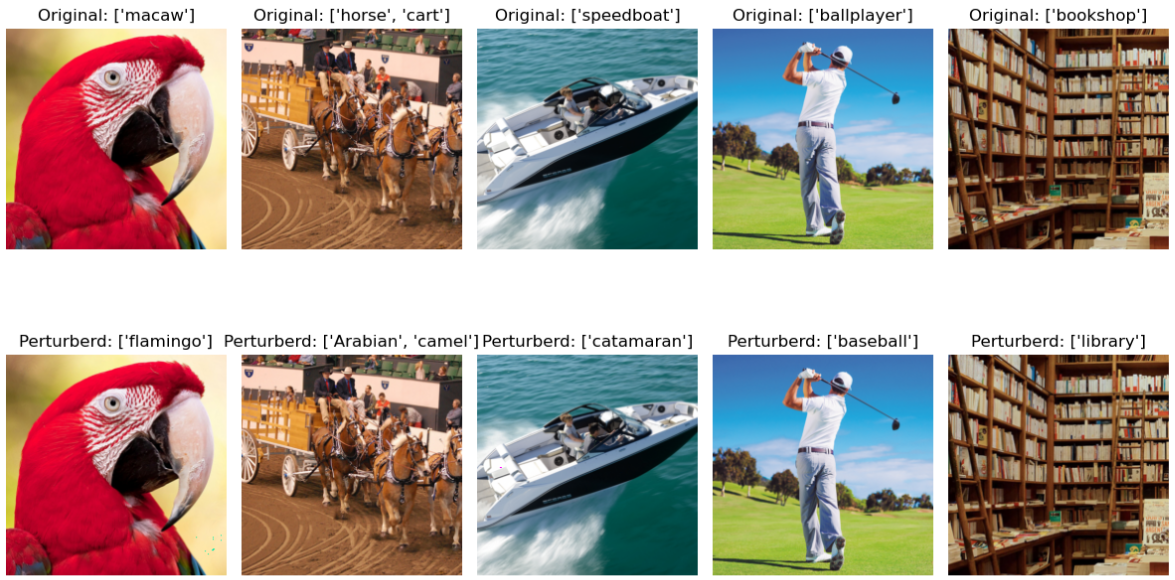
\includegraphics[width=1\linewidth]{results/result_pert_global.png}
    \caption{Results of the deepfool algorithm on 5 images classified by ResNet34}
    \label{fig:result_global_deepfool}
\end{figure}

The perturbations are almost to totally imperceptible for the human eye. If we look closely, it's possible to see some alterations, like a red patch of pixel on the back of the boat in the third image. By observing in more details the perturbations, it's possible to see that different images will be perturbed in totally differents manners. For example, we can see on figure \ref{fig:diff_global_grey} that some images, like the third one, will be very locally altered but quite intensely, while other images like the fifth one will be globally altered but with little intensity.

\begin{figure}[H]
    \centering
    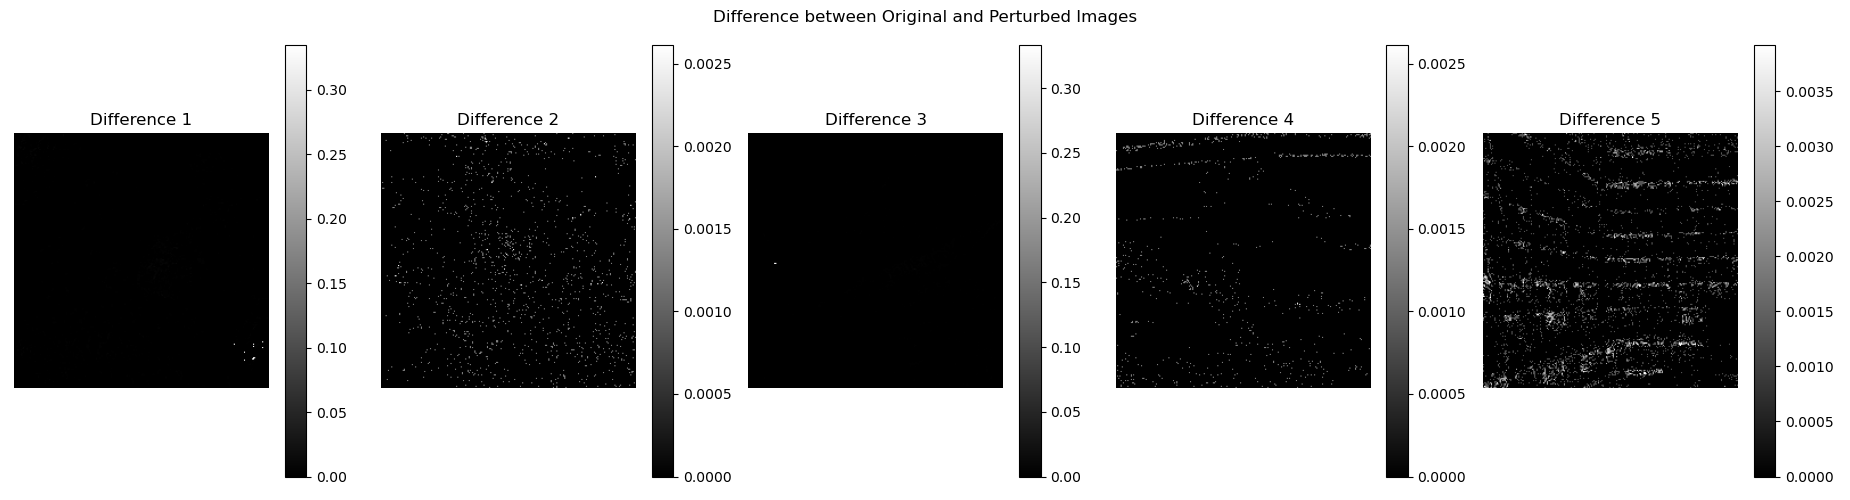
\includegraphics[width=1\linewidth]{results/Diff_global_rescal.png}
    \caption{Perturbations applied by the algorithm to the five test images (original pixel values were scaled from 0 to 1)}
    \label{fig:diff_global_grey}
\end{figure}

\newpage
\section{Localised Deepfool}

We have reworked DeepFool to apply it in a localized manner on the image. We started by selecting a specific region of the image and then enforcing a transformation on that particular area. The new equation used to compute minimal perturbation restricted to a region $R$ can then be written as follow :

\begin{equation}
	r_*(x_0) = \frac{|f_{\hat{l}(x_0)}(x_0) - f_k(x_0)|}{\|w_{\hat{l}(x_0)} - w_k\|_{2,R}^2} (w_{\hat{l}(x_0)} - w_k)^R
\end{equation}

The algorithm still works this way, but sometimes will need to alter greatly the given region to fool the classification. On the first image of figure \ref{fig:vs_50-80}, we can for example clearly see the chosen region for perturbation.

\begin{figure}[H]
    \centering
    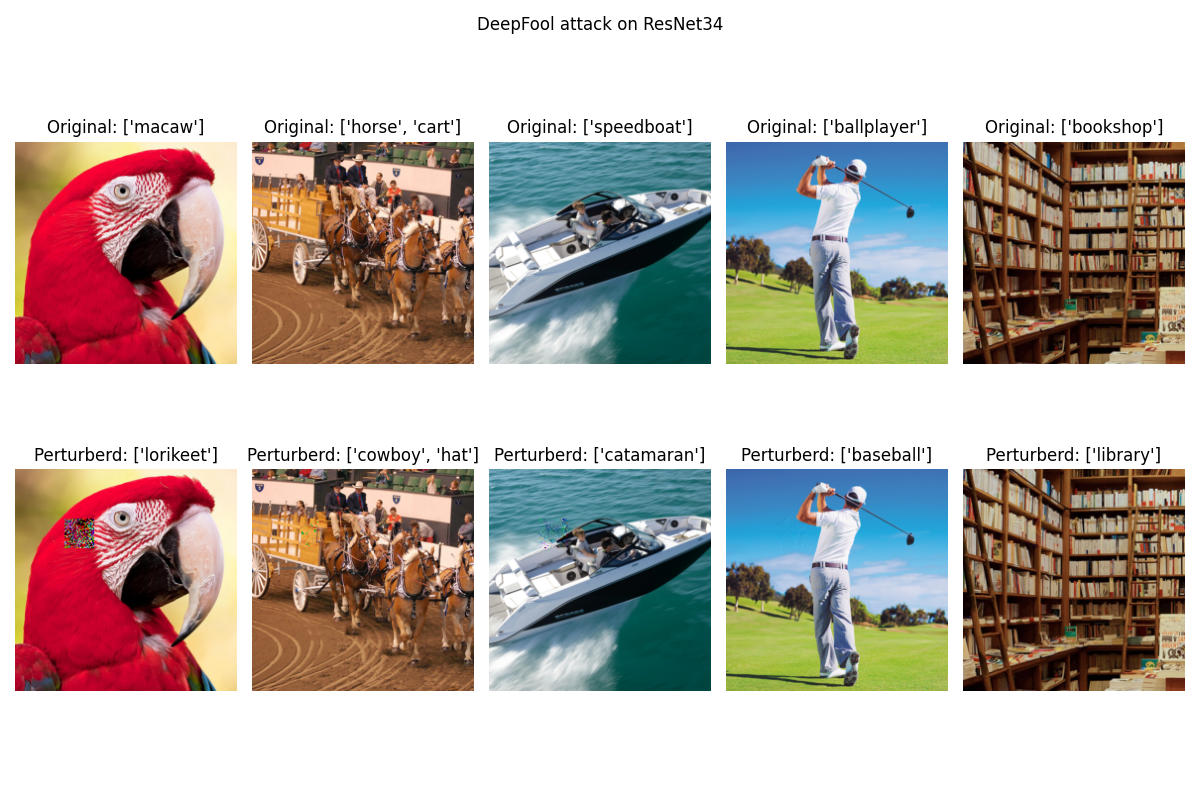
\includegraphics[width=1\linewidth]{results/vs_50-80.png}
    \caption{Results of the deepfool algorithm restrained on a local area on 5 images classified by ResNet34}
    \label{fig:vs_50-80}
\end{figure}

Compared to generalised DeepFool which can perturb images without it being perceptible every time, the application of the localised Deepfool to a randomly selected restricted area of the image can significantly affects the algorithm's performance. The image of the macaw becomes heavily degraded when DeepFool is applied specifically to the selected region in this experiment.

\begin{figure}[H]
    \centering
    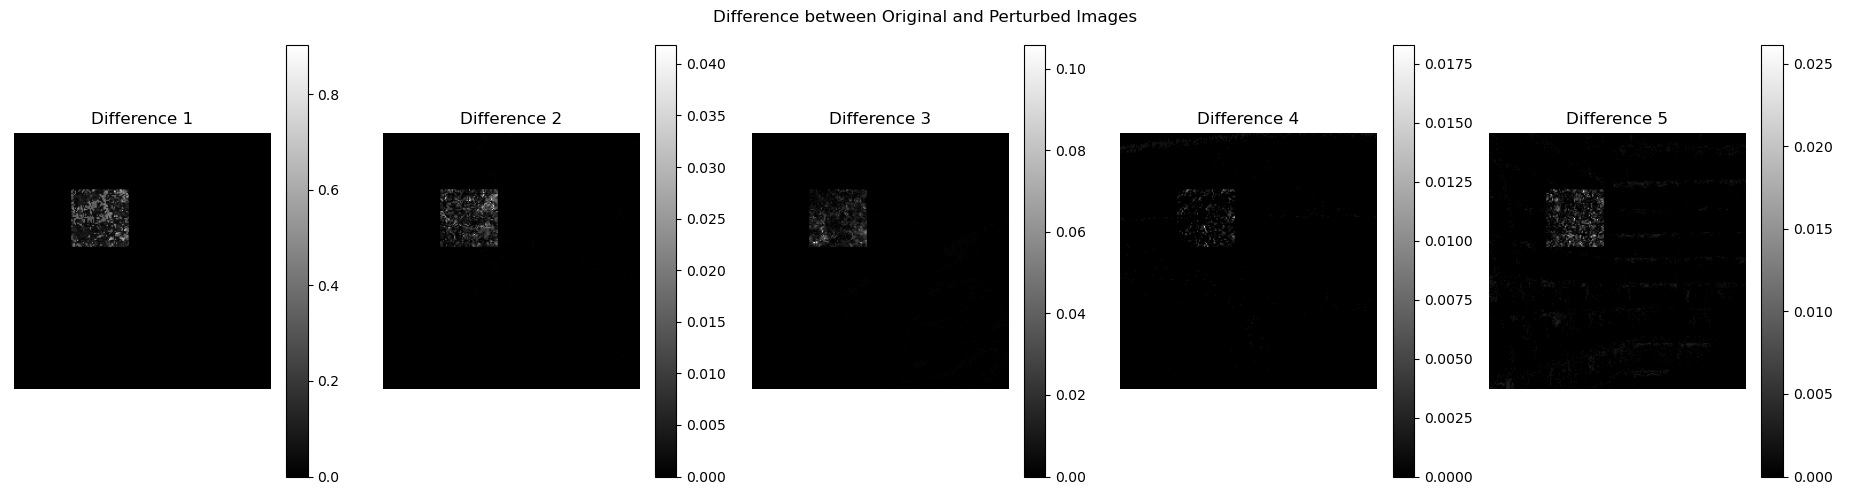
\includegraphics[width=1\linewidth]{results/Diff_local_grey.png}
    \caption{Perturbations applied localy by the algorithm to the five test images (original pixel values were scaled from 0 to 1)}
    \label{fig:diff_local_grey}
\end{figure}


We then asked ourselves if there are specific areas in an image that should be prioritised for optimal degradation. To explore this, we divided each image using a 4x4 grid and applied localized DeepFool on each grid cell. The results for the macaw image show that certain areas are clearly more effective for perturbation, as illustrated in Figure \ref{fig:max_1}. 

\begin{figure}[H]
    \centering
    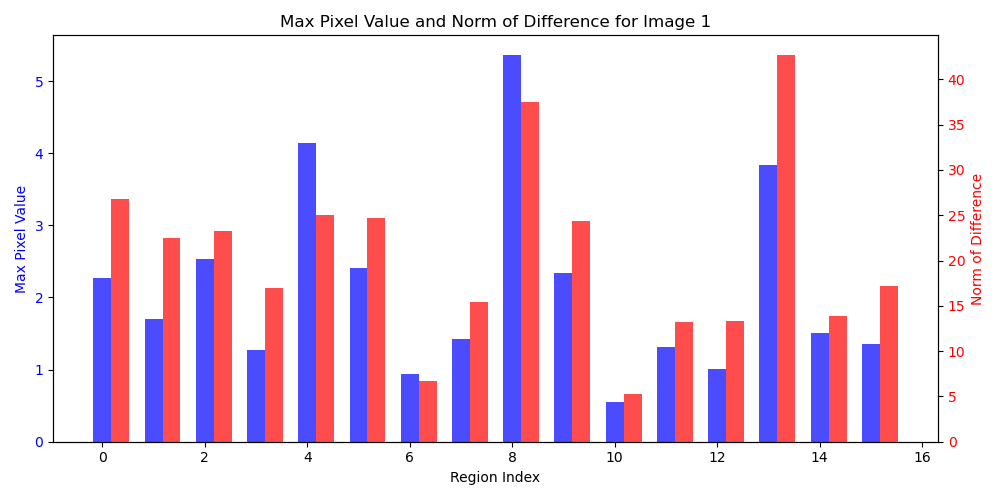
\includegraphics[width=1\linewidth]{results/max_value_pixel_norm_diff_1.png}
    \caption{}
    \label{fig:max_1}
\end{figure}

Those results are similar for the other images, and so it should be possible to develop an algorithm that tries to minimize not only the norm of the perturbation but also its size for any images. That could be used to find more localised perturbation that could be used in cases like the hat that makes faces of people being misclassified.

\newpage
\section{Universal perturbation}

The general idea behind universal perturbation is trying to get a perturbation that can be applied to any images given as input to a model, and fool the model most of the time. This perturbation is considered "universal" because it can be applied regardless of the image and original classification of the image perturbed.\\

The algorithm will iterate on many images and apply the Deepfool algorithm on it, and each time update the perturbation with the results of Deepfool. The maximum norm authorized is set beforehand, so the perturbation can be controlled to not alter the image too much. When the perturbation can fool the model at a chosen minimum rate, the algorithm stops and returns the actual perturbation.

\begin{figure}[H]
    \centering
    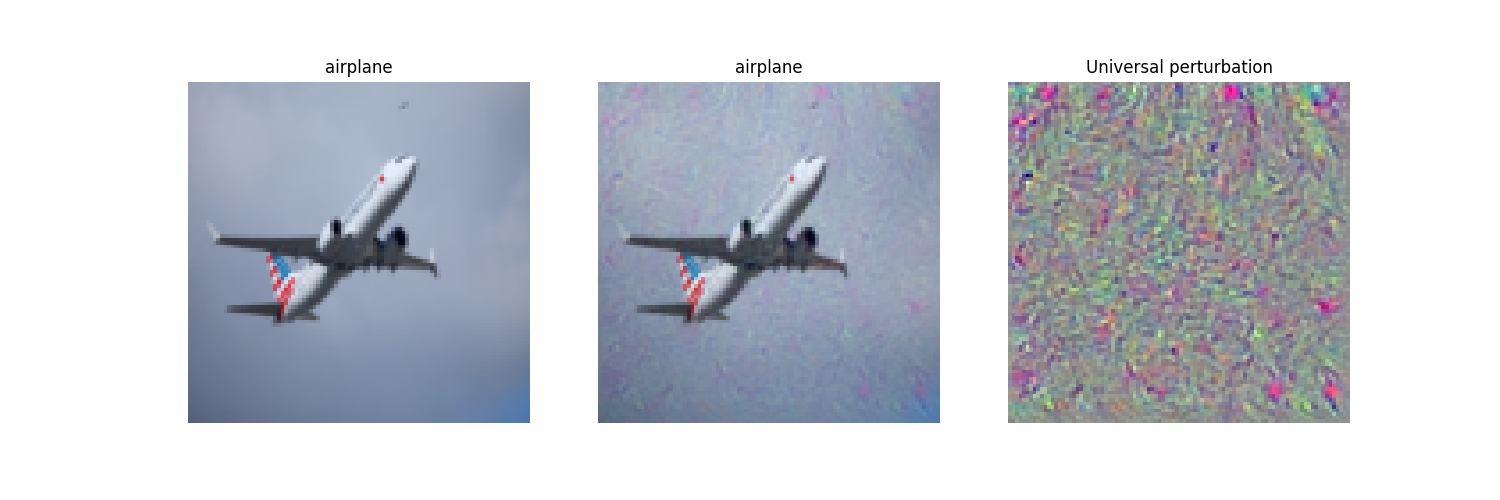
\includegraphics[width=1\linewidth]{results/example_universal_stl10_resnet.png}
    \caption{Results of a universal perturbation applied on the dataset stl10 classified by ResNet}
    \label{fig:universal}
\end{figure}

On figure \ref{fig:universal}, we can see the results of our implementation of universal perturbation on the stl10 dataset classified by a fine-tuned version of ResNet. The perturbation fools the model 40\% of the time, which is the goal we set for the algorithm to get results in a satisfying time. 

% comparaison de la perturbation avec random perturb pour voir les fool rate ?

\section{Image Detection}

We have tested YOLO for image detection, on both live video and pictures. 
This represents a first step towards the next phase of the project, where we will attempt to deceive classifiers on live video streams.


\begin{figure}[ht]
    \begin{minipage}[t]{0.49\textwidth}
        \centering
        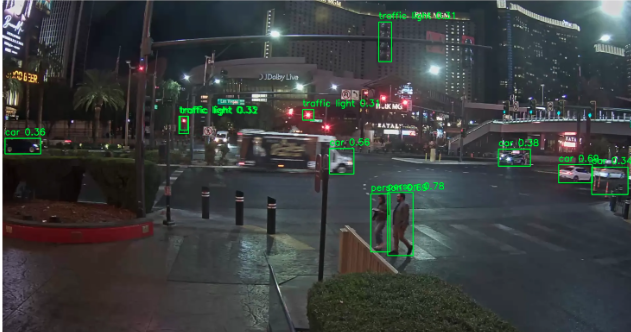
\includegraphics[width=\textwidth]{results/YOLO-Video.png}
        \caption{Use of YOLO on live video}
        \label{fig:Yolo Video}
    \end{minipage}
    \hfill
    \begin{minipage}[t]{0.49\textwidth}
        \centering
        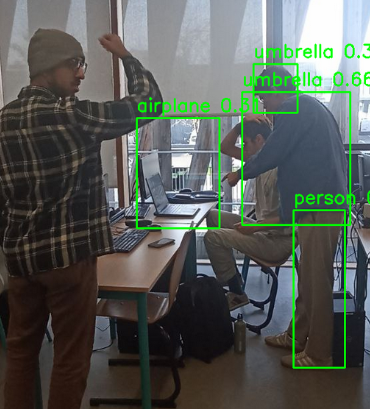
\includegraphics[width=0.5\textwidth]{results/YOLO-Photo.png}
        \caption{Use of YOLO on a picture}
        \label{fig:Yolo Photo}
    \end{minipage}
\end{figure}

\section{Next Steps}

From now on we'll try to shift our focus to real-time detection, and see how we can alter the vision of models like Yolo. The goal is to have similar results as the ones on the presentation of the project, like the hoodie that makes people invisible.

While doing so, we'll also try to explore a little the possibilities with the algorithms we have already implemented, for example to compare the efficiency of a same perturbation on differents models, or try using universal perturbation with the localised Deepfool algorithm to see if its possible to have acceptable universal results with a localised perturbation.


\end{document}